% CS-370 OEL report -- IEEE conference format. Compile:  pdflatex report && pdflatex report
% Tables come from tables.tex, regenerated by `python run_all.py` (experiments/make_report_tables.py).
\documentclass[conference]{IEEEtran}
\usepackage{graphicx,booktabs,amsmath,amssymb,url}
\extrafloats{60}
\graphicspath{{../../results/}}
\newcommand{\stamp}{Rameen Kashif (456834) \textbar{} Manal Aslam (465734) \textbar{} Zainab Ali Bangash (486688)}

\begin{document}
\title{An Autonomous Delivery Agent under Slip, Theft and Rival-Triggered Flooding\\
\large CS-370 Open Ended Lab, instance 6a18af32}
\author{\IEEEauthorblockN{Rameen Kashif (456834), Manal Aslam (465734), Zainab Ali Bangash (486688)}
\IEEEauthorblockA{\stamp}}
\maketitle

\begin{abstract}
We build a delivery agent for a $23\times23$ grid city with four terrain costs, teleport
tunnels, a blocker rival that steals parcels, slip probability 0.12 and our approved third
twist, rival-triggered flooding. We formulate the tour as one search problem over
(position, delivered/stolen mask, flood countdown), implement six search algorithms from
scratch and design a tunnel-aware heuristic that we prove admissible and verify consistent on
every edge of the state space. The rival interaction is played as a reduced game with
Minimax and Alpha-Beta; our move ordering saves 91\% of Minimax nodes at depth~5. A Claude
dispatcher drives the planners through four tools behind a validation layer. All numbers are
reproduced by \texttt{python run_all.py} from our CMS IDs.
\end{abstract}

\section{Instance and Agent Formalisation (Part A)}
The instructor's generator gives grid size 23, obstacle density 0.24, terrain costs road 1,
grass 2, mud 3, ford 8 (36 fords), depot $(8,7)$ and stops S1 $(21,5)$, S2 $(0,1)$, S3
$(22,17)$, S4 $(15,18)$; S3 is itself a ford. Tunnels are placed by us, seeded from the
instance hash: $(0,5)\leftrightarrow(9,2)$, $(12,0)\leftrightarrow(13,10)$,
$(12,4)\leftrightarrow(12,17)$ (Fig.~\ref{fig:map}). The vectorised cost map is 7.3$\times$
faster than a Python loop at $23\times23$ and $\approx$45$\times$ at $184\times184$.
PEAS, the environment classification (fully observable, stochastic, sequential, dynamic,
discrete, competitive multi-agent) and the choice of a utility-based agent are in
\texttt{docs/part\_a\_analysis.md}; we summarise them in Table~I of that file.
% TODO(group): paste the PEAS table here (short form) if space allows.

\begin{figure}[t]\centering
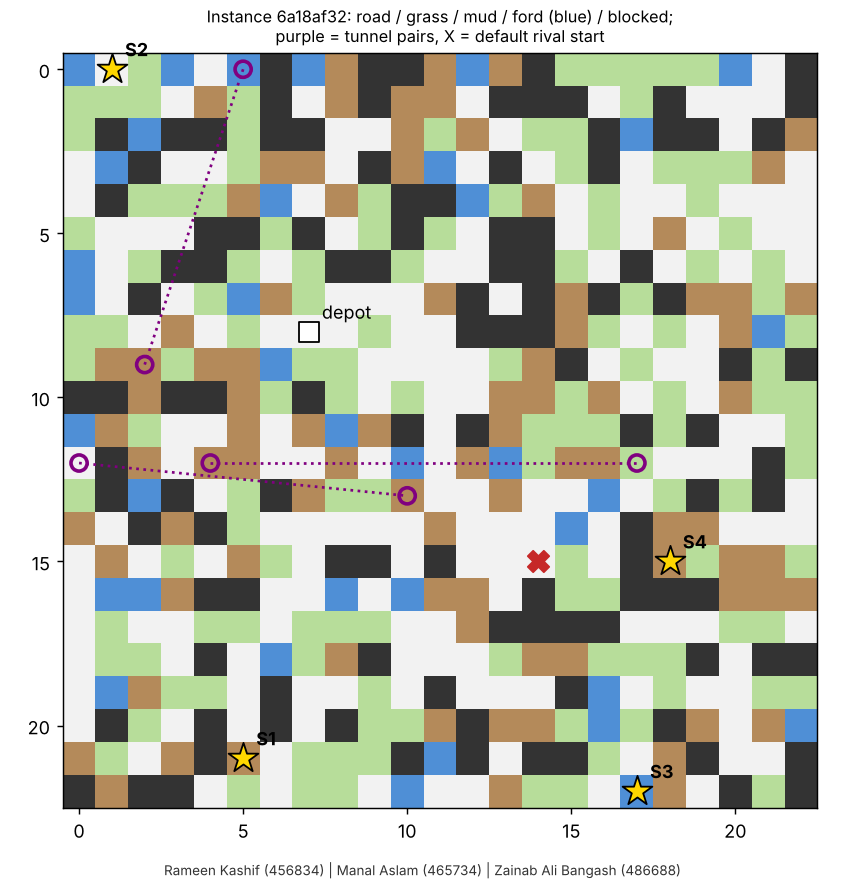
\includegraphics[width=0.8\columnwidth]{instance_map.png}
\caption{Instance 6a18af32: terrain, tunnel pairs, stops, depot and default rival start.}
\label{fig:map}\end{figure}

\section{Route Planning (Part B)}
\subsection{Search problem}
A state is $(p, m, \phi)$: position, a 4-bit mask of stops delivered \emph{or stolen}, and the
remaining flooded steps $\phi$. Because time only matters while the fords are under water, the
countdown replaces the raw time step and bounds the space by $529\cdot16\cdot(F+1)$. Actions
are the four moves (cost of the cell entered), \textsc{Tunnel} (cost 1) and \textsc{Wait}
(cost 1, only while flooded). The goal is $m = 1111_2$.

\subsection{Heuristic $h_{\text{tunnel-mst}}$}
On a complete graph over the stops and tunnel mouths we put Manhattan$\times c_{\min}$ edges
plus cost-1 tunnel edges, and take shortest paths $d^*$. For remaining stops $R$,
\begin{equation}
h(p,m) = \min_{x\in R} d^*(p,x) + \mathrm{MST}_{d^*}(R).
\end{equation}
\emph{Admissibility.} $d^*$ is a relaxation (no walls, every cell at $c_{\min}$, no flood), so
$d^*\le$ true cost; any route from $p$ reaches a first stop and then visits the rest along a
spanning path of $R$, whose weight is at least the MST. \emph{Consistency.} Our first version
used $\mathrm{MST}(\{p\}\cup R)$; an exhaustive check found 674 violating edges (deleting a
degree-2 point can shorten an MST). Attaching $p$ by its cheapest edge removes all violations
(0 over all 418 cells $\times$ 16 masks $\times$ successors) and is never weaker. The full proof
is in \texttt{docs/part\_b\_heuristic.md}.

% generated by experiments/make_report_tables.py -- Rameen Kashif (456834) | Manal Aslam (465734) | Zainab Ali Bangash (486688)

\begin{table}[t]
\centering
\footnotesize
\caption{Search algorithms (1-stop variant and full tour).}
\label{tab:alg}
\setlength{\tabcolsep}{3pt}
\begin{tabular}{lrrrrrrr}
\toprule
problem & alg. & cost & steps & expanded & stored & mem KB & ms \\
\midrule
depot-$>$S4 & BFS & 30.0 & 12 & 165 & 195 & 16.9 & 2.91 \\
depot-$>$S4 & UCS & 26.0 & 12 & 275 & 316 & 51.2 & 6.41 \\
depot-$>$S4 & DLS(l=12) & 30.0 & 12 & 7142 & 60 & 3.7 & 167.99 \\
depot-$>$S4 & IDS & 30.0 & 12 & 34003 & 60 & 3.8 & 812.22 \\
depot-$>$S4 & Greedy & 30.0 & 12 & 12 & 30 & 7.2 & 0.89 \\
depot-$>$S4 & A$^*$ & 26.0 & 12 & 128 & 161 & 40.0 & 4.86 \\
full tour & BFS & 132.0 & 51 & 4123 & 4281 & 863.7 & 95.86 \\
full tour & UCS & 111.0 & 61 & 5187 & 5330 & 1854.3 & 233.91 \\
full tour & Greedy & 132.0 & 51 & 64 & 129 & 41.5 & 4.05 \\
full tour & A$^*$ & 111.0 & 61 & 3436 & 3772 & 1735.8 & 158.99 \\
full tour & IDS & inf & 0 & 550597 & 75 & 5.3 & 12932.76 \\
\bottomrule
\end{tabular}
\end{table}

\begin{table}[t]
\centering
\footnotesize
\caption{Heuristics with A* on the full tour (optimal cost 111).}
\label{tab:heur}
\setlength{\tabcolsep}{3pt}
\begin{tabular}{lrrrrrr}
\toprule
heuristic & h(s0) & cost & expanded & ms & viol. & Greedy \\
\midrule
tunnel\_mst & 47.0 & 111.0 & 3436 & 226.6 & 0 & 132.0 \\
mst\_plain & 60.0 & 116.0 & 2877 & 187.9 & 14 & 172.0 \\
nearest & 14.0 & 116.0 & 4395 & 453.4 & 25 & 172.0 \\
farthest & 24.0 & 116.0 & 3968 & 291.4 & 26 & 166.0 \\
sum\_dstar & 56.0 & 113.0 & 3061 & 253.5 & 1308 & 157.0 \\
zero & 0.0 & 111.0 & 5187 & 257.9 & 0 & 119.0 \\
\bottomrule
\end{tabular}
\end{table}

\begin{table}[t]
\centering
\footnotesize
\caption{Admissibility on 150 sampled states (h* from UCS).}
\label{tab:adm}
\setlength{\tabcolsep}{3pt}
\begin{tabular}{lrrrr}
\toprule
heuristic & samples & h$>$h$^*$ & max h/h$^*$ & mean h/h$^*$ \\
\midrule
tunnel\_mst & 150 & 0 & 0.792 & 0.458 \\
mst\_plain & 150 & 1 & 1.061 & 0.573 \\
nearest & 150 & 1 & 1.061 & 0.277 \\
farthest & 150 & 1 & 1.061 & 0.423 \\
sum\_dstar & 150 & 0 & 0.792 & 0.502 \\
\bottomrule
\end{tabular}
\end{table}

\begin{table}[t]
\centering
\footnotesize
\caption{Inadmissible / faster variants and their cost gap.}
\label{tab:inadm}
\setlength{\tabcolsep}{3pt}
\begin{tabular}{lrrrrr}
\toprule
variant & cost & expanded & time\_ms & gap & gap \% \\
\midrule
A$^*$ + tunnel\_mst (optimal) & 111.0 & 3436 & 163.3 & 0.0 & 0.0 \\
A$^*$ + sum\_dstar & 113.0 & 3061 & 139.0 & 2.0 & 1.8 \\
WA$^*$ w=2 + tunnel\_mst & 111.0 & 709 & 40.0 & 0.0 & 0.0 \\
WA$^*$ w=3 + tunnel\_mst & 119.0 & 95 & 6.1 & 8.0 & 7.2 \\
Greedy + tunnel\_mst & 132.0 & 64 & 5.8 & 21.0 & 18.9 \\
\bottomrule
\end{tabular}
\end{table}

\begin{table}[t]
\centering
\footnotesize
\caption{Memory limit (stored-node cap), depot to S4.}
\label{tab:mem}
\setlength{\tabcolsep}{3pt}
\begin{tabular}{lrrrrrr}
\toprule
node cap & A$^*$ ok & A$^*$ stored & IDS ok & IDS stored & IDS expanded & IDS ms \\
\midrule
25 & False & 27 & False & 26 & 189 & 3.8 \\
50 & False & 51 & False & 51 & 12627 & 300.4 \\
100 & False & 101 & True & 60 & 34003 & 908.7 \\
200 & True & 161 & True & 60 & 34003 & 810.0 \\
400 & True & 161 & True & 60 & 34003 & 810.1 \\
800 & True & 161 & True & 60 & 34003 & 838.4 \\
\bottomrule
\end{tabular}
\end{table}

\begin{table}[t]
\centering
\footnotesize
\caption{Nodes per decision, Minimax vs Alpha-Beta.}
\label{tab:nodes}
\setlength{\tabcolsep}{3pt}
\begin{tabular}{lrrrrrr}
\toprule
d & root & MM & AB & AB+ord & saved & saved+ord \\
\midrule
2 & agent (MAX) & 31 & 20 & 16 & 36.4 & 50.4 \\
2 & rival (MIN) & 32 & 21 & 20 & 35.5 & 37.1 \\
3 & agent (MAX) & 145 & 58 & 45 & 60.0 & 68.9 \\
3 & rival (MIN) & 165 & 79 & 59 & 52.1 & 64.0 \\
4 & agent (MAX) & 733 & 168 & 103 & 77.1 & 85.9 \\
4 & rival (MIN) & 746 & 208 & 134 & 72.1 & 82.0 \\
5 & agent (MAX) & 3267 & 482 & 258 & 85.2 & 92.1 \\
5 & rival (MIN) & 3655 & 662 & 319 & 81.9 & 91.3 \\
\bottomrule
\end{tabular}
\end{table}

\begin{table}[t]
\centering
\footnotesize
\caption{Weight grid search (top 6 of 18).}
\label{tab:tune}
\setlength{\tabcolsep}{3pt}
\begin{tabular}{lrrrrrr}
\toprule
race & ford & mobility & margin & wins & mean cost & score \\
\midrule
0.0 & 0.0 & 0.25 & -0.25 & 1 & 201.1 & -0.6522 \\
0.0 & 6.0 & 0.25 & -0.25 & 1 & 201.2 & -0.6525 \\
2.0 & 0.0 & 0.25 & -0.25 & 1 & 202.3 & -0.6547 \\
0.0 & 15.0 & 0.25 & -0.25 & 1 & 206.1 & -0.6622 \\
5.0 & 0.0 & 0.0 & -0.5 & 1 & 134.3 & -0.7687 \\
5.0 & 6.0 & 0.0 & -0.5 & 1 & 134.3 & -0.7687 \\
\bottomrule
\end{tabular}
\end{table}

\begin{table}[t]
\centering
\footnotesize
\caption{30 games vs the blocker (Wilson 95\% CI).}
\label{tab:games}
\setlength{\tabcolsep}{3pt}
\begin{tabular}{lrrrrr}
\toprule
config & win & draw & loss & delivered & stolen \\
\midrule
Alpha-Beta agent (d=3), tuned & 0.13 [0.05, 0.30] & 0.60 [0.42, 0.75] & 0.27 [0.14, 0.44] & 1.7 $\pm$ 0.3 & 1.9 $\pm$ 0.2 \\
Alpha-Beta agent (d=3), default & 0.13 [0.05, 0.30] & 0.63 [0.46, 0.78] & 0.23 [0.12, 0.41] & 1.7 $\pm$ 0.3 & 1.9 $\pm$ 0.3 \\
A$^*$ planner agent & 0.13 [0.05, 0.30] & 0.60 [0.42, 0.75] & 0.27 [0.14, 0.44] & 1.9 $\pm$ 0.2 & 2.1 $\pm$ 0.2 \\
\bottomrule
\end{tabular}
\end{table}

\begin{table}[t]
\centering
\footnotesize
\caption{Slip and replanning (planner, no rival; deterministic plan 111).}
\label{tab:slip}
\setlength{\tabcolsep}{3pt}
\begin{tabular}{lrrrrrr}
\toprule
slip p & replans & slips & extra cost & extra \% & steps & finished \\
\midrule
0.0 & 0.0 $\pm$ 0.0 & 0.0 & 0.0 $\pm$ 0.0 & 0.0 & 61.0 & 30 \\
0.12 & 9.3 $\pm$ 1.4 & 9.3 & 24.4 $\pm$ 5.6 & 22.0 & 73.6 & 30 \\
0.3 & 32.3 $\pm$ 3.2 & 32.3 & 82.4 $\pm$ 9.4 & 74.2 & 105.0 & 30 \\
0.5 & 83.4 $\pm$ 7.6 & 83.4 & 203.4 $\pm$ 16.6 & 183.2 & 165.6 & 27 \\
\bottomrule
\end{tabular}
\end{table}

\begin{table}[t]
\centering
\footnotesize
\caption{Dispatcher success over 20 requests (claude-haiku-5-5).}
\label{tab:llm}
\setlength{\tabcolsep}{3pt}
\begin{tabular}{lrrr}
\toprule
method & runs & success & mean tool calls \\
\midrule
direct planner call & 20 & 1.00 [0.84, 1.00] & 1.3 \\
LLM (validated) & 0 & not run (no key, no cache) &  \\
LLM (raw) & 0 & not run (no key, no cache) &  \\
\bottomrule
\end{tabular}
\end{table}

\begin{table}[t]
\centering
\footnotesize
\caption{30 scenarios per configuration (mean $\pm$ 95\% CI).}
\label{tab:configs}
\setlength{\tabcolsep}{3pt}
\begin{tabular}{lrrrrr}
\toprule
config & win rate & delivered & stolen & cost & replans \\
\midrule
A$^*$ planner (naive) & 0.13 [0.05,0.30] & 1.87 $\pm$ 0.23 & 2.13 $\pm$ 0.23 & 134.80 $\pm$ 15.72 & 15.60 $\pm$ 3.19 \\
A$^*$ planner (flood-aware) & 0.13 [0.05,0.30] & 1.63 $\pm$ 0.35 & 2.37 $\pm$ 0.35 & 130.80 $\pm$ 11.93 & 14.87 $\pm$ 2.97 \\
Alpha-Beta agent (tuned) & 0.13 [0.05,0.30] & 1.67 $\pm$ 0.28 & 1.90 $\pm$ 0.25 & 167.27 $\pm$ 30.42 & 8.10 $\pm$ 1.37 \\
Alpha-Beta, rival has no dam & 0.10 [0.03,0.26] & 1.43 $\pm$ 0.27 & 2.13 $\pm$ 0.27 & 172.80 $\pm$ 34.23 & 7.03 $\pm$ 1.25 \\
Alpha-Beta, no stealing & 0.93 [0.79,0.98] & 1.37 $\pm$ 0.33 & 0.00 $\pm$ 0.00 & 257.70 $\pm$ 16.74 & 3.17 $\pm$ 0.94 \\
\bottomrule
\end{tabular}
\end{table}

\begin{table}[t]
\centering
\footnotesize
\caption{Flood duration sweep.}
\label{tab:flood}
\setlength{\tabcolsep}{3pt}
\begin{tabular}{lrrrrr}
\toprule
config & win rate & delivered & stolen & cost & dam used \\
\midrule
flood\_duration=0 & 0.17 [0.07,0.34] & 1.53 $\pm$ 0.32 & 2.00 $\pm$ 0.31 & 182.43 $\pm$ 35.85 & 7 \\
flood\_duration=10 & 0.17 [0.07,0.34] & 1.50 $\pm$ 0.31 & 1.93 $\pm$ 0.28 & 192.27 $\pm$ 38.29 & 26 \\
flood\_duration=15 & 0.13 [0.05,0.30] & 1.67 $\pm$ 0.28 & 1.90 $\pm$ 0.25 & 167.27 $\pm$ 30.42 & 28 \\
flood\_duration=25 & 0.13 [0.05,0.30] & 1.57 $\pm$ 0.29 & 1.83 $\pm$ 0.26 & 188.53 $\pm$ 35.27 & 28 \\
\bottomrule
\end{tabular}
\end{table}

\begin{table}[t]
\centering
\footnotesize
\caption{Heuristic ablation on 30 random stop sets.}
\label{tab:abl}
\setlength{\tabcolsep}{3pt}
\begin{tabular}{lrrrrr}
\toprule
heuristic & A$^*$ expanded & cost & time ms & suboptimal runs & mean gap \\
\midrule
tunnel\_mst & 1735 $\pm$ 350 & 74.3 $\pm$ 7.4 & 22.1 $\pm$ 4.7 & 0 & 0.0 \\
mst\_plain & 1415 $\pm$ 319 & 74.6 $\pm$ 7.4 & 14.3 $\pm$ 3.2 & 4 & 0.37 \\
nearest & 2929 $\pm$ 339 & 74.7 $\pm$ 7.3 & 29.9 $\pm$ 6.7 & 4 & 0.4 \\
zero & 3968 $\pm$ 374 & 74.3 $\pm$ 7.4 & 22.0 $\pm$ 2.1 & 0 & 0.0 \\
\bottomrule
\end{tabular}
\end{table}


\subsection{Results}
Table~\ref{tab:alg} compares the algorithms. BFS and IDS minimise the number of actions, not
cost (132 vs.\ 111 on the full tour). A$^*$ with our heuristic returns the optimal 111 and
expands 3436 nodes against 5187 for UCS. IDS is exponential in depth: it solves 1-stop
variants (depth 11--17) but is stopped after 500k expansions on the 61-action tour.
Table~\ref{tab:heur} shows the key finding of the heuristic study: \emph{the handout's
Manhattan baselines are inadmissible on our map}, because a tunnel jump costs 1 while covering
up to 21 Manhattan units. A$^*$ with \texttt{nearest}, \texttt{farthest} or \texttt{mst\_plain}
(our heuristic without tunnels) returns 116, not 111 (Table~\ref{tab:adm} shows the sampled
overestimates). \textbf{Inadmissible but faster} (Table~\ref{tab:inadm}): weighted A$^*$ with
$w=3$ expands 95 nodes (36$\times$ fewer) and returns 119 (+7.2\%); greedy returns 132 (+18.9\%).
\textbf{Memory limit} (Table~\ref{tab:mem}): with a cap of 100 stored nodes A$^*$ fails on
depot$\to$S4 while IDS, which only keeps the current path and its successor lists and rejects
children already on that path, still succeeds.

\section{The Rival (Part C)}
The game alternates agent (MAX) and blocker (MIN) plies; the agent is confined to a $7\times7$
window, the blocker has four moves, \textsc{Wait} and a single \textsc{OpenDam}, steals any
undelivered stop it enters and blocks the cell it stands on. Leaves are scored by
\begin{equation}
E = w_1 f_{\text{tour}} + w_2 f_{\text{score}} + w_3 f_{\text{race}} + w_4 f_{\text{ford}} + w_5 f_{\text{mob}},
\end{equation}
defined and justified in \texttt{docs/part\_c\_eval.md}. Two design lessons: an admissible lower
bound in $f_{\text{tour}}$ makes \textsc{Wait} look best (the agent stalled), so we use the exact
static remaining-tour cost; and features that jump between neighbouring cells (per-cell ford
dependence, ``next stop'' race) create cliffs that also cause stalls, so both were smoothed.
Our ordering (Table~\ref{tab:nodes}) raises pruning at depth 5 from 82--85\% to 91--92\%, with
values identical to Minimax. Weight tuning is a grid search over 18 weight vectors
(Table~\ref{tab:tune}); Table~\ref{tab:games} reports 30 games with Wilson intervals.
Table~\ref{tab:slip} shows the cost of slip: at $p=0.12$ the planner replans $\approx$9 times
and pays $\approx$22\% above the deterministic plan; at $p=0.5$ the overhead exceeds 180\%.
% TODO(group): 2-3 sentences interpreting Table tab:games (draws dominate; why).

\section{LLM Dispatcher (Part D)}
Claude (\texttt{claude-haiku-5-5}) calls \texttt{plan\_route}, \texttt{simulate},
\texttt{flood\_status} (our twist) and \texttt{tunnel\_info} in a manual ReAct loop. The
validation layer checks names, stop ids, terrain, step ranges and obviously infeasible
constraints before execution and returns an error observation otherwise. Twenty requests
range from single plans to infeasible ones (avoid fords while S3 is a ford; avoid mud, which
encloses the depot; cost $<100$; a non-existent S5). Table~\ref{tab:llm} compares the direct
planner call with the LLM with and without validation; traces and the Sense--Reason--Act
mapping are in \texttt{results/llm\_traces/} and \texttt{docs/part\_d\_llm.md}.
% TODO(group): after the keyed run, describe the logged errors (wrong tool / invented args /
% ignored constraints) and include two traces.

\section{Integration and Evaluation (Part E)}
The Streamlit UI (\texttt{streamlit run app.py}) shows the grid, tunnels, flood state, plan,
agent and rival and exposes every viva parameter. Each configuration is run on the same 30
scenarios seeded by $\mathrm{sha256}(\text{``scenario}|\text{6a18af32}|i\text{''})$, which fix
the rival start and the slip draws (Table~\ref{tab:configs}, Fig.~\ref{fig:configs}).
Table~\ref{tab:flood} sweeps the flood duration. The \textbf{ablation} (Table~\ref{tab:abl})
removes the tunnel edges from our heuristic: it expands fewer nodes but returns a suboptimal
tour on some of the 30 random stop sets, i.e.\ the tunnel component is what keeps the
heuristic admissible. \textbf{Failure analysis} (\texttt{results/part\_e\_scenarios.json},
\texttt{failures}): losses come from rival starts next to a stop, thefts during a flood and
stand-offs. Without stealing the blocker learns to stand \emph{on} the stop the agent is
heading for, which the rules make impassable; a rule forbidding the rival from occupying a
stop would be needed.
% TODO(group): interpret Tables tab:configs and tab:flood.

\begin{figure}[t]\centering
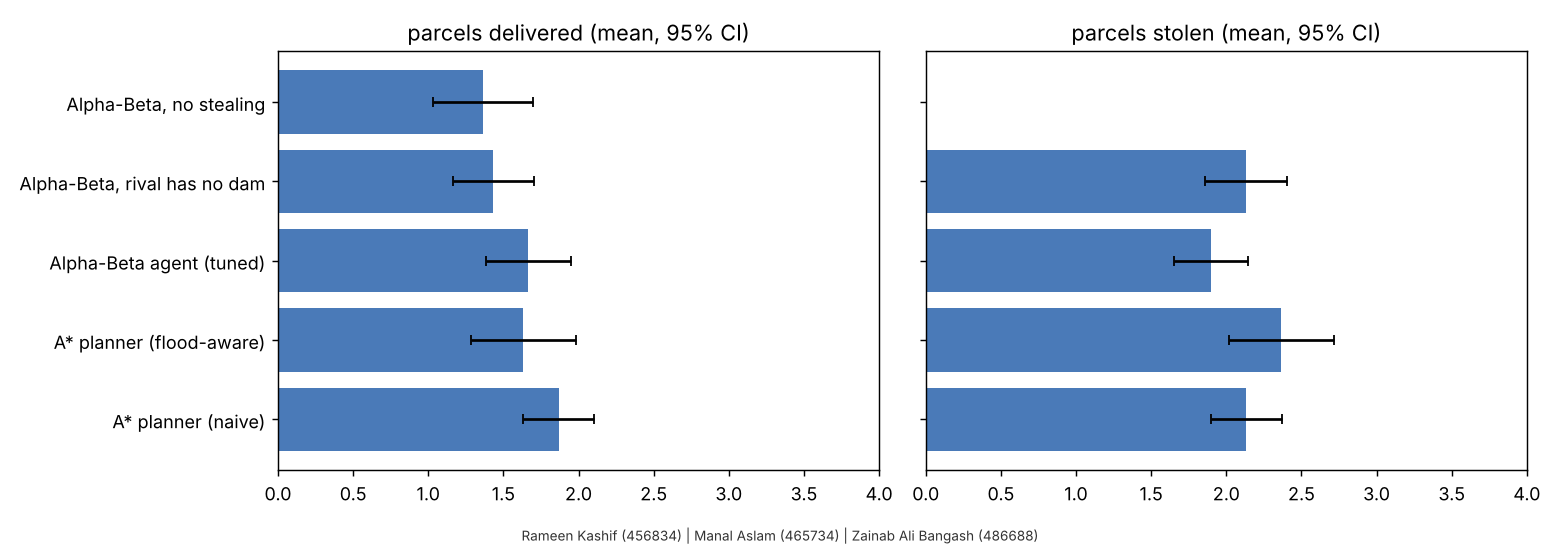
\includegraphics[width=\columnwidth]{part_e_configs.png}
\caption{Parcels delivered and stolen per configuration (30 scenarios, 95\% CI).}
\label{fig:configs}\end{figure}

\section{Ethics and Reflection}
% Half a page; source: docs/ethics_reflection.md
Wrong decisions affect customers (late or lost parcels), road users (a robot sent across a
flooded ford because the planner assumed deterministic motion), the operator who carries the
liability, and staff whose work is planned around the robot. An LLM dispatcher can sound
confident while ignoring a constraint. Our safeguards: validation before execution, the LLM
can only call tested planners, infeasibility must be reported, uncertainty is simulated with
replanning, and every number and LLM response is seeded or cached for audit. Our own errors
(an inconsistent first heuristic, stalling evaluation features, baselines that silently became
inadmissible) were each found by exhaustive testing rather than by derivation.

\section*{Reproducibility}
\texttt{python run_all.py} regenerates every table (\texttt{docs/report/tables.tex}) and figure
(\texttt{results/}). Every output carries the stamp: \stamp.

\end{document}
